\documentclass[12pt,a4paper]{report}

\usepackage[brazil]{babel}
\usepackage[utf8]{inputenc}

\usepackage{graphicx}

\title{Especificações do Projeto SIGEST}
\author{Taciano Morais Silva - tacianosilva@gmail.com}

\begin{document}

\maketitle
\listoffigures
\tableofcontents

\chapter{Introdução}

Texto de introdução para testar a citação \cite{morais04a}.

\section{Definição de Perfis}

No sistema teremos vários tipos de usuário e seus respectivos perfis.
Segue abaixo a lista de usuários do sistema e seus respecitivos perfis. 

\emph{Professor} - Entidade que representa o professor que pode assumir um dos
seguintes perfis:

\begin{itemize}
\item Coordenador de Curso
\item Coordenador de Estágio
\item Avaliador de Estágio
\item Orientador de Estágio
\end{itemize}

\emph{Administrador} - Entidade que representa o super usuário que pode
assumir um dos seguintes perfis:

\begin{itemize}
\item Administrador
\item Super Administrador
\end{itemize}

\chapter{Projeto Arquitetural}

\chapter{Modelo de Dados}

% Figura Modelo de Dados
\begin{figure}[!htb]
        \centering
        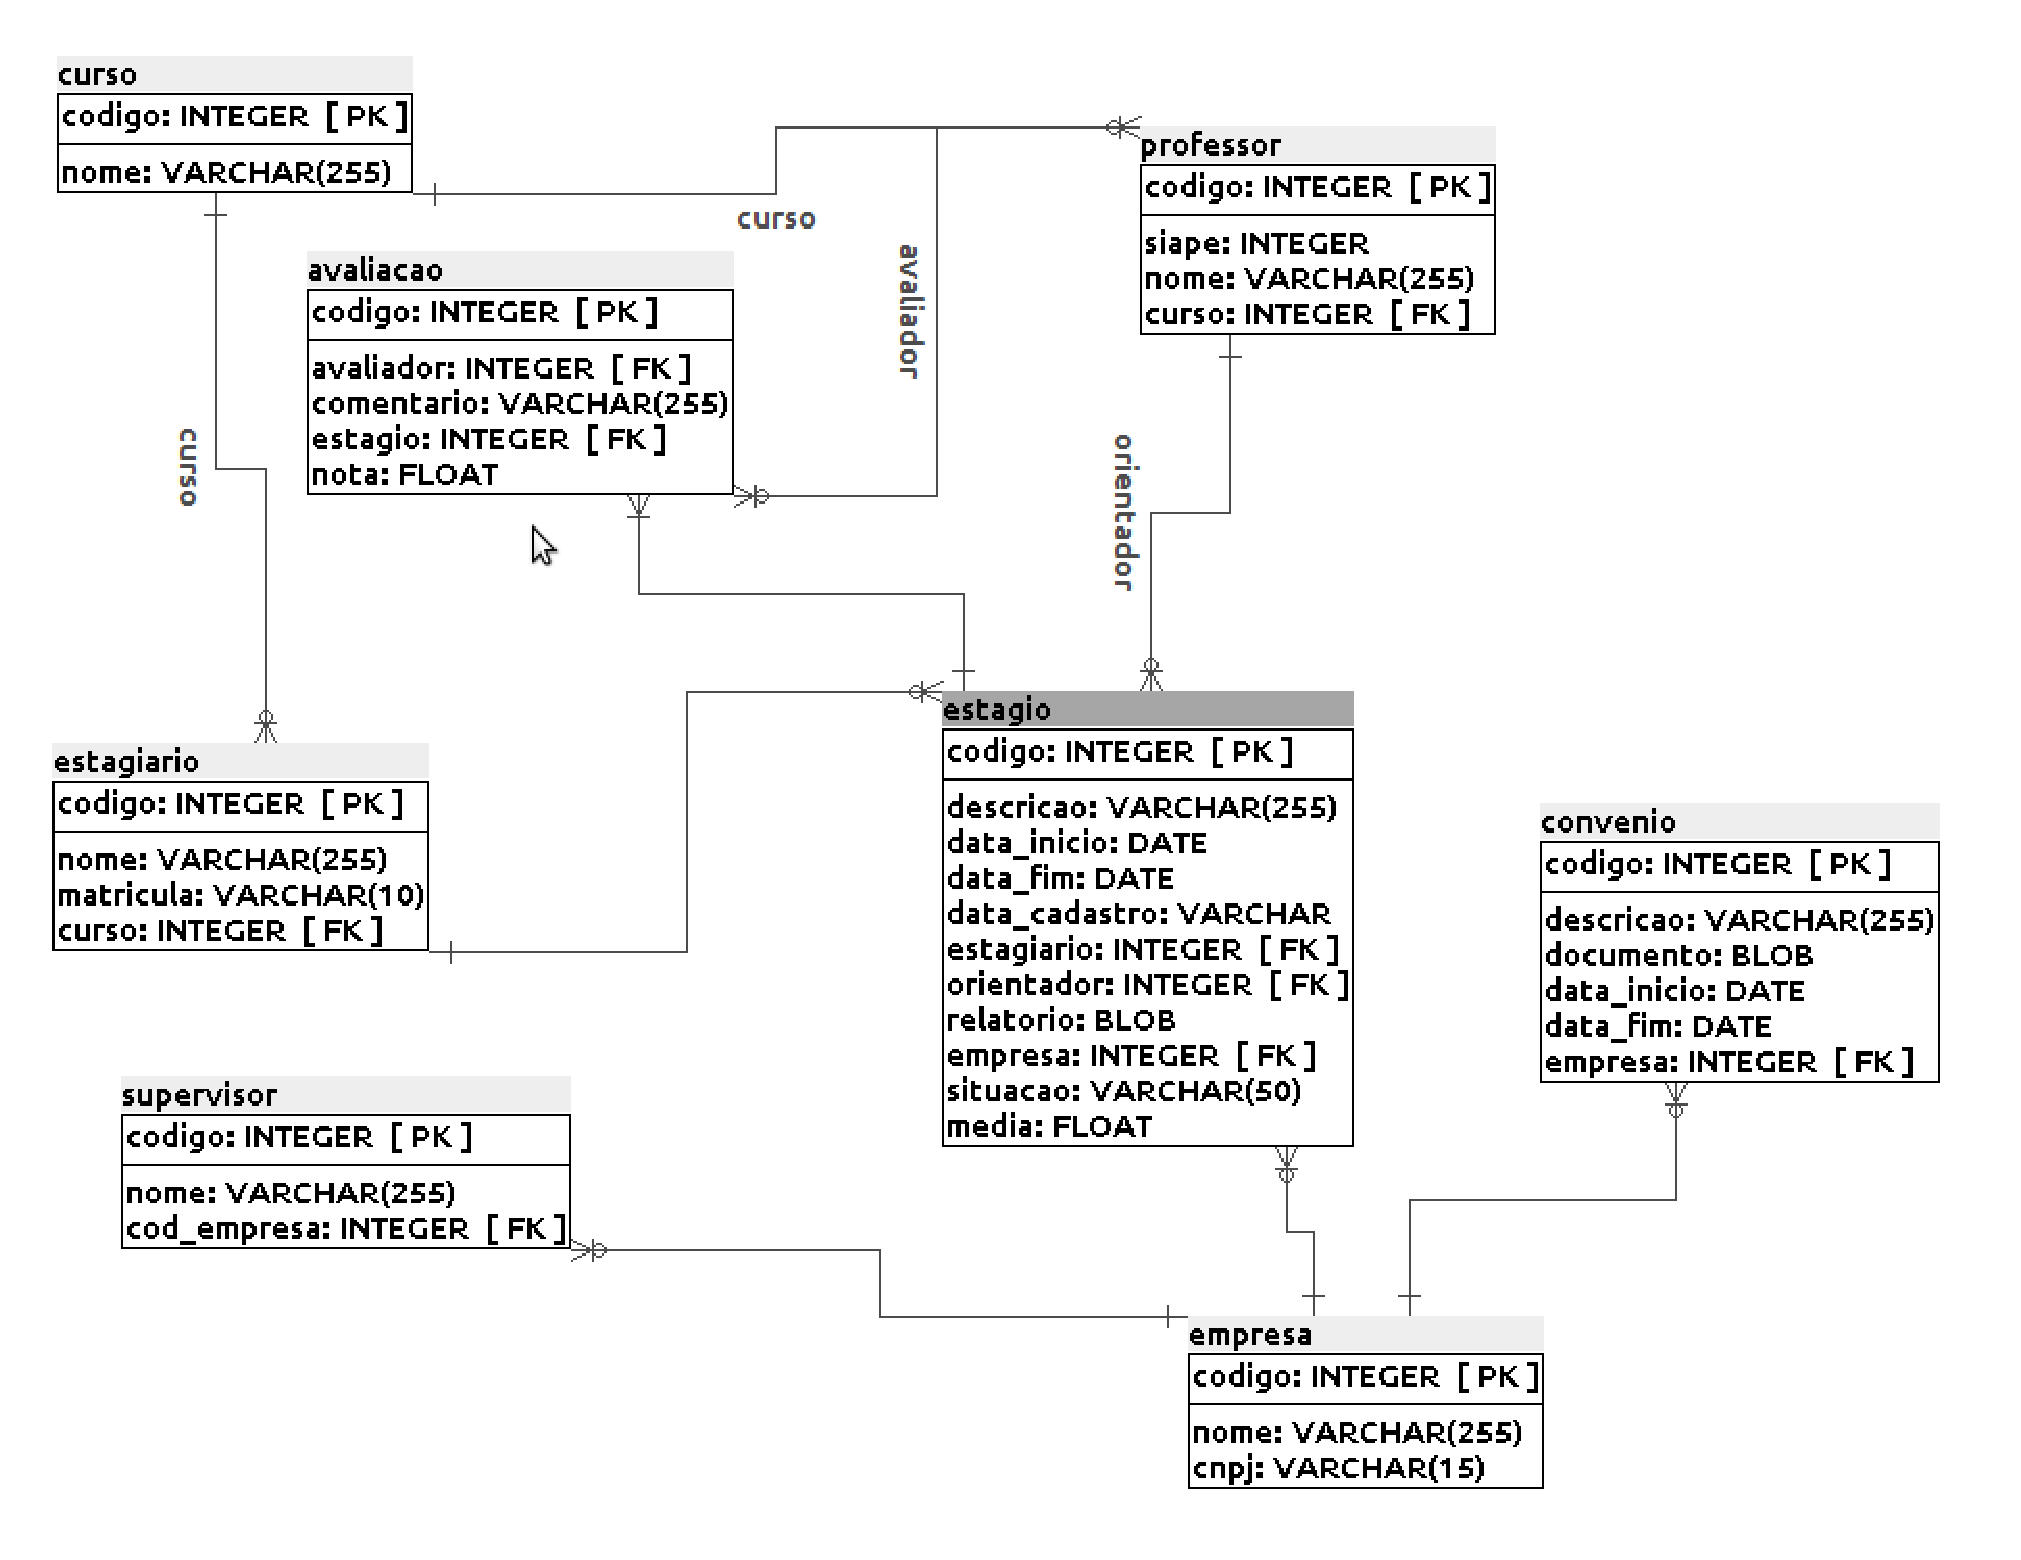
\includegraphics[scale=0.4]{esquema_sigest.eps}
        \caption{Esquema Relacionado para o Sistema SIGEST}
        \label{esquema_sigest}
\end{figure}
%\footnote{"A framework is a set of classes that embodies an abstract design for solutions to a family of related problems", \cite{johnson88}}


\chapter{Lista de Casos de Uso}

%% Input para a Section CDU001 - Estagiário
\section{CDU01 - Estagiário}

\subsection{Responsável}

Nome: Fladson

GitHub:

\subsection{Descrição}

\subsection{Fluxo Principal}

\subsection{Fluxo Secundário}

\subsection{Fluxo de Exceção}

\subsection{Diagrama de Classe}

\subsection{Diagrama de Sequência}

\section{CDU02 - Estágio}

\subsection{Responsável}

Nome: Aragon

GitHub:

\subsection{Descrição}

\subsection{Fluxo Principal}

\subsection{Fluxo Secundário}

\subsection{Fluxo de Exceção}

\subsection{Diagrama de Classe}

\subsection{Diagrama de Sequência}

\section{CDU03 - Empresa}

\subsection{Responsável}

Nome: Alisson

GitHub:

\subsection{Descrição}

\subsection{Fluxo Principal}

\subsection{Fluxo Secundário}

\subsection{Fluxo de Exceção}

\subsection{Diagrama de Classe}

\subsection{Diagrama de Sequência}

\section{CDU04 - Professor}

\subsection{Responsável}

Nome: Mércia

GitHub:

\subsection{Descrição}

\subsection{Fluxo Principal}

\subsection{Fluxo Secundário}

\subsection{Fluxo de Exceção}

\subsection{Diagrama de Classe}

\subsection{Diagrama de Sequência}

\section{CDU005 - Curso}

\subsection{Responsável}

Dados do responsável pela documentação:

Nome: Taciano

GitHub: tacianosilva

\subsection{Descrição}
A entidade \emph{Curso}, será a responsável por representar e armazenar as
características de um curso que receberá alunos para estágios.

Um \emph{Curso} possui as seguintes características:

\begin{itemize}
  \item código: Numérico tipo serial;
  \item nome: Texto tipo varchar;
  \item coordenador: Numérico tipo serial - código de um professor;
  \item vice coordenador: Numérico tipo serial - código de um professor;
  \item coordenador de estágios: Numérico tipo serial - código de um professor;
  \item resolução de estágios: Binário - tipo  blob para enviar um pdf;
  \item fórmulários avaliativos para os estágios (voluntários ou obrigatórios);
\end{itemize}

A entidade Curso terá relacionamentos com as seguintes entidades:

\begin{itemize}
  \item Estágios de alunos do curso;
  \item Coordenador do curso - um professor;
  \item Vice coordenador do curso - um professor;
  \item Coordenador de estágios - um professor; 
\end{itemize}
 
\subsection{Fluxo Principal}

Dependendo dos atores a entidade curso poderá ser acessada de formas diferentes.
Temos os seguintes atores possíveis: Professor, Coordenador, Aluno Estagiário e
Supervisor.

\subsubsection{Incluir Curso}

Para incluir um curso o ator segue os seguintes passos:

\begin{itemize}
  \item O ator faz login no sistema;
  \item O sistema verifica se o ator tem permissão para a função (apenas
  administradores);
  \item O sistema abre a tela para cadastrar um novo curso;
  \item O ator preenche os dados do curso;
  \item O ator salva o novo curso; 
\end{itemize}


\subsubsection{Alterar Curso}

\begin{itemize}
  \item O ator faz login no sistema;
  \item O sistema verifica se o ator tem permissão para a função (apenas
  administradores);
  \item O sistema abre a tela para alterar o curso;
  \item O ator preenche os dados do curso;
  \item O ator salva as alterações curso; 
\end{itemize}

\subsubsection{Consultar Curso}

\begin{itemize}
  \item O ator faz login no sistema;
  \item O sistema verifica se o ator tem permissão para a função (apenas
  administradores);
  \item O sistema abre a tela para consultar e listar os cursos; 
\end{itemize}

\subsection{Fluxo Secundário}

\subsubsection{Consultar Estágios do Curso}

\begin{itemize}
  \item O ator faz login no sistema;
  \item O sistema verifica se o ator tem permissão para a função;
  \item O sistema abre a tela para consultar e listar os cursos;
  \item O ator define as informações de filtragem;
  \item O sistema apresenta a lista de estágios do curso; 
\end{itemize}

\subsection{Fluxo de Exceção}

\subsection{Diagrama de Classe}

\subsection{Diagrama de Sequência}

%%%%%%%%%%%%%%%%%%%%%%%%%%%%%%%%%%%%%%%%%%%%%%%%%%%%%%%%%%%%%%%%%%%%%%%%%%%%%%%
%% Bibliografia

\bibliographystyle{alpha} % estilo de bibliografia
\bibliography{bib-dis} % arquivos com as entradas bib.

%%%%%%%%%%%%%%%%%%%%%%%%%%%%%%%%%%%%%%%%%%%%%%%%%%%%%%%%%%%%%%%%%%%%%%%%%%%%%%%
%% Ap\^endice
 % Caso seja necessário algum apêndice, descomente a próxima linha.

%\appendix

%\input{capA-filosofos}

\end{document}
